% !TeX spellcheck = en_US
\documentclass[12pt]{article}
\usepackage[utf8]{inputenc}
\usepackage[spanish]{babel}
\usepackage{graphicx}
\usepackage[margin=2.5cm]{geometry}
\usepackage{float}
\usepackage{amsmath}
\usepackage{amsfonts}
\newcommand{\hrules}{\rule{\linewidth}{0.5mm}}

\begin{document}
	
	\begin{titlepage}
		\centering
		
		\begin{minipage}{0.2\textwidth}
			\begin{flushleft}
				
\includegraphics[width=\textwidth]{logo_ipn.png}
			\end{flushleft}
		\end{minipage}
		\hfill
		\begin{minipage}{0.5\textwidth}
			\centering
			{\scshape\Large Instituto Politécnico Nacional} \\[0.3cm]
			{\scshape\large Escuela Superior de Cómputo}
		\end{minipage}
		\hfill
		\begin{minipage}{0.2\textwidth}
			\begin{flushright}
				
\includegraphics[width=\textwidth]{logo_escom.png}
			\end{flushright}
		\end{minipage}
		
		\vspace{1.5cm}
		
		{\large\textbf{Ingeniería en Inteligencia Artificial}} \\[1.5cm]
		
		{\Large\textbf{Redes Neuronales y Aprendizaje Profundo}} \\[2cm]
		
		\hrules
		\vspace{0.4cm}
		{\huge\bfseries 
			Práctica 1: Perceptron Multicapa y Clasificación
		} \\[0.4cm]
		\hrules
		\vspace{2.5cm}
		
		% --- INFORMACIÓN PERSONAL ---
		\begin{minipage}{0.8\textwidth}
			\begin{flushleft} \large
				\textbf{Profesor:} \\
				Saul de la O Torres 
				\\[1cm]
				
				\textbf{Alumno:} \\
				Velázquez Arrieta Eduardo Uriel
			\end{flushleft}
		\end{minipage}
		
		\vfill
		
		{\large Fecha de entrega:  11 de Septiembre 2026}
		
	\end{titlepage}
	
	
	\newpage
	\tableofcontents % Índice de contenido
	\vspace{1cm}
	
	\listoffigures    % Índice de imágenes
	\newpage
	
	
	\section{Introducción}
	El campo de la Inteligencia Artificial (IA) abarca diversas disciplinas orientadas a modelar y resolver problemas complejos mediante la automatización del razonamiento y el aprendizaje computacional. Dentro del aprendizaje automático (\textit{Machine Learning}), los problemas se estructuran principalmente en tres grandes paradigmas: clasificación (asignación de categorías discretas), regresión (predicción de valores continuos) y agrupamiento (\textit{clustering}, segmentación por similitud). Si bien estos enfoques resultan sumamente eficientes en múltiples aplicaciones cotidianas, históricamente han mostrado limitaciones al intentar replicar los mecanismos subyacentes del procesamiento cognitivo y sensorial humano ante tareas aparentemente intuitivas.
	
	Para comprender la evolución que condujo a los modelos modernos de aprendizaje profundo (\textit{Deep Learning}), es fundamental estudiar los cimientos teóricos de las redes neuronales artificiales. El punto de partida histórico se remonta al modelo formal de la neurona artificial de McCulloch-Pitts y al perceptrón propuesto por Frank Rosenblatt, cuyo objetivo inicial consistía en modelar funciones lógicas básicas y resolver problemas de discriminación binaria mediante hiperplanos separadores.
	
	A nivel conceptual, el análisis de compuertas lógicas como \textbf{AND}, \textbf{OR} y \textbf{XOR} ilustra la limitación fundamental de los perceptrones de una sola capa:
	
	\begin{itemize}
		\item{\textbf{Compuerta AND y OR}: Representan problemas linealmente separables. Sus tablas de verdad pueden dividirse geométricamente en el plano mediante una única línea recta (un hiperplano de dimensión 1), permitiendo que un perceptrón simple ajuste sus pesos sin dificultad.}
		
		\begin{figure}[h!]
			\centering
			\begin{tabular}{|c|c|c|}
				\hline
				A & B & X \\
				\hline
				0   &   0 &  0   \\
				\hline
				0   &   1    &  0   \\
				\hline
				1   &   0  &  0    \\ 
				\hline 
				1 & 1 & 1 \\
				\hline
			\end{tabular}
			\caption{Tabla de verdad de la compuerta AND.}
			\label{fig:compuerta-and}
		\end{figure}
		
		Al graficar las entradas de la compuerta AND, se observa que una función lineal del tipo $y = -x + \frac{3}{2}$ separa de manera exacta la clase $0$ de la clase $1$.
		
		\begin{figure}[H]
			\centering
			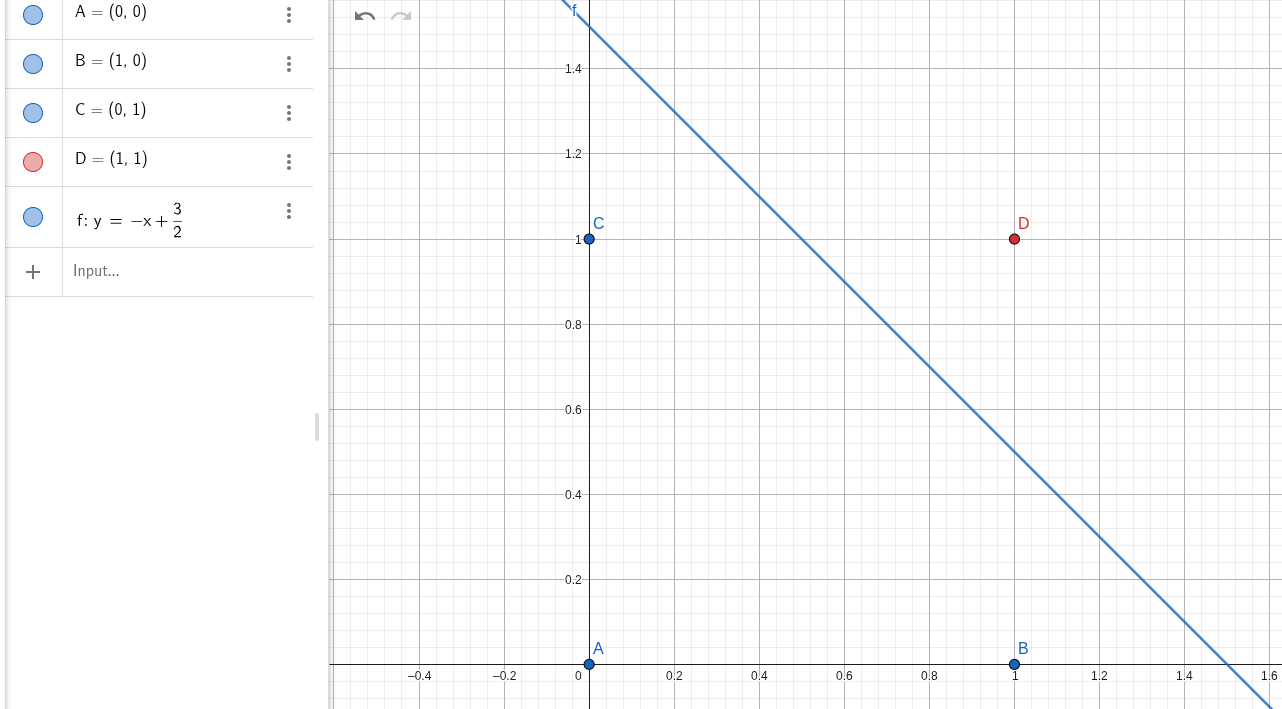
\includegraphics[width=0.7\textwidth]{img1.png} 
			\caption{Separabilidad lineal en la compuerta AND.}
			\label{fig:esquema_1}
		\end{figure}   
		
		\item{\textbf{Compuerta OR}: Al igual que la anterior, admite una solución lineal mediante el ajuste del sesgo o frontera con una función como $y = -x + \frac{1}{2}$.}
		
		\begin{figure}[h!]
			\centering
			\begin{tabular}{|c|c|c|}
				\hline
				A & B & X \\
				\hline
				0   &   0 &  0   \\
				\hline
				0   &   1    &  1  \\
				\hline
				1   &   0  &  1    \\ 
				\hline 
				1 & 1 & 1 \\
				\hline
			\end{tabular}
			\caption{Tabla de verdad de la compuerta OR.}
			\label{fig:compuerta-or}
		\end{figure}
		
		\begin{figure}[H]
			\centering
			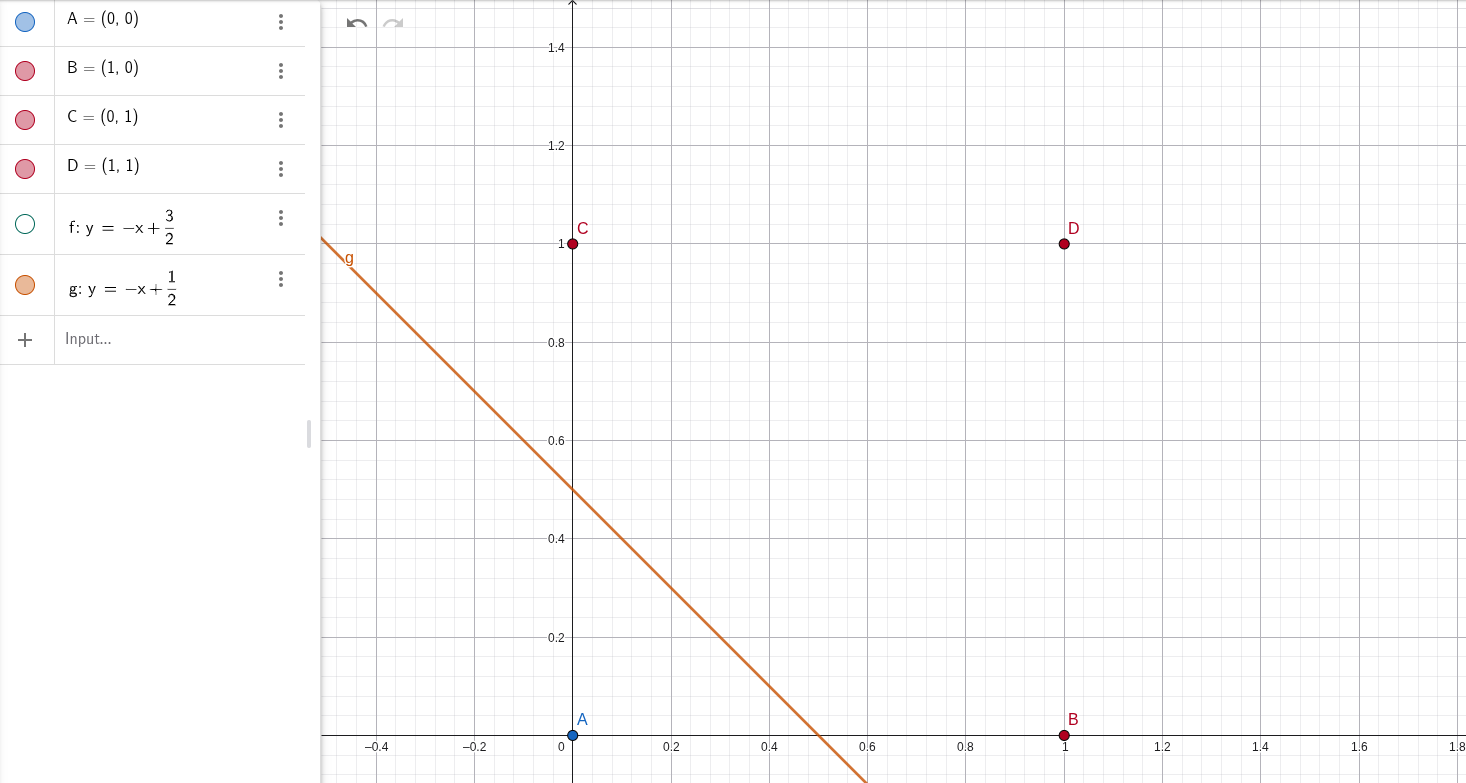
\includegraphics[width=0.7\textwidth]{img2.png} 
			\caption{Separabilidad lineal en la compuerta OR.}
			\label{fig:esquema_2}
		\end{figure}
		
		\newpage	
		\item{\textbf{Compuerta XOR}: Representa un problema no linealmente separable. Como se demostró en la literatura clásica de Minsky y Papert, un perceptrón simple es incapaz de resolver la función XOR debido a que los puntos de clases opuestas se entrelazan de tal forma que se requieren múltiples líneas de decisión (o capas ocultas) para lograr su clasificación.}
		
		\begin{figure}[h!]
			\centering
			\begin{tabular}{|c|c|c|}
				\hline
				A & B & X \\
				\hline
				0   &   0 &  0   \\
				\hline
				0   &   1    &  1  \\
				\hline
				1   &   0  &  1    \\ 
				\hline 
				1 & 1 & 0 \\
				\hline
			\end{tabular}
			\caption{Tabla de verdad de la compuerta XOR.}
			\label{fig:compuerta-xor}
		\end{figure}
		
		La imposibilidad de trazar un único hiperplano motivó la transición hacia arquitecturas capaces de aprender fronteras de decisión complejas, sentando las bases para el estudio de problemas multiclase del mundo real, tales como la clasificación del conjunto de datos \textbf{Iris} (compuesto por las especies \textit{Setosa}, \textit{Versicolor} y \textit{Virginica}).
		
		\begin{figure}[H]
			\centering
			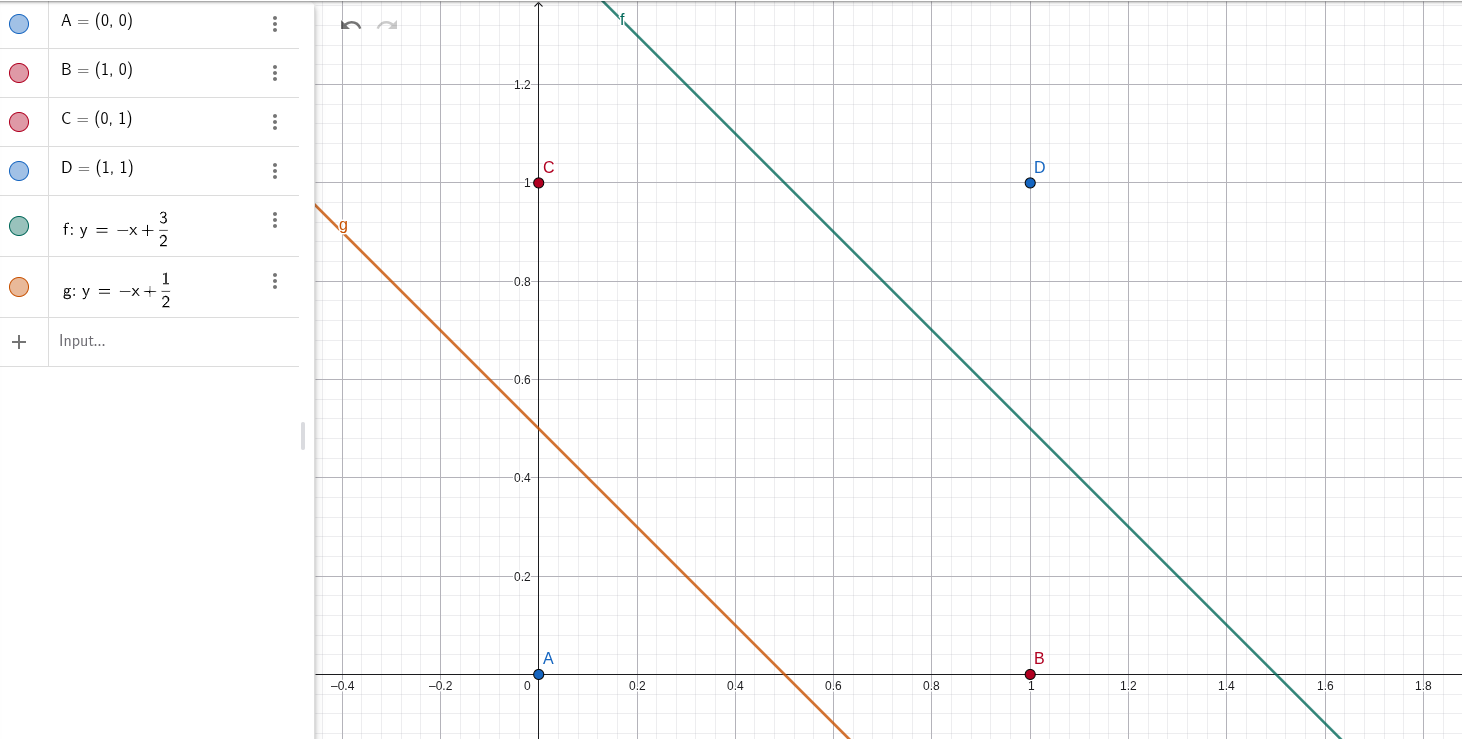
\includegraphics[width=0.7\textwidth]{img3.png} 
			\caption{Incapacidad de separación lineal simple en la compuerta XOR.}
			\label{fig:esquema_3}
		\end{figure}
	\end{itemize}
	
	\newpage
	\section{Desarrollo Experimental}
	
	El propósito central de esta práctica es diseñar, implementar y evaluar arquitecturas de redes neuronales utilizando dos de los frameworks computacionales más potentes y adoptados en la industria y la investigación científica:
	\begin{enumerate}
		\item \textbf{TensorFlow}: Desarrollado por Google, destaca por su robustez en producción y su API de alto nivel orientada a la definición flexible de grafos y modelos orientados a objetos.
		\item \textbf{PyTorch}: Desarrollado por Meta, sobresale por su paradigma de grafos dinámicos y su uso intensivo de tensores con diferenciación automática (\textit{Autograd}), facilitando la depuración y el diseño modular.
	\end{enumerate}
	
	Para evaluar el comportamiento de ambos entornos, se emplea el clásico conjunto de datos \textbf{Iris}. Este dataset se compone de vectores de cuatro características morfológicas estandarizadas:
	
	\begin{figure}[h!]
		\centering
		\begin{tabular}{|c|c|c|c|c|}
			\hline
			A & B & C & D & X \\
			\hline
		\end{tabular}
		\caption{Estructura del vector de características de entrada.}
		\label{fig:vector_caracteristicas}
	\end{figure}
	
	\begin{itemize}
		\item A: Longitud del sépalo (\textit{Sepal Length}) 	
		\item B: Ancho del sépalo (\textit{Sepal Width}) 
		\item C: Longitud del pétalo (\textit{Petal Length})
		\item D: Ancho del pétalo (\textit{Petal Width})
		\item X: Clase o etiqueta de la especie botánica (\textit{Setosa, Versicolor, Virginica})
	\end{itemize}
	
	El conjunto de datos consta de 150 instancias en total (50 por cada una de las tres clases). Adicionalmente, se integra un conjunto de validación independiente de 15 muestras nunca antes vistas por los modelos, permitiendo medir de forma rigurosa la capacidad de generalización fuera de muestra.
	
	\begin{figure}[H]
		\centering
		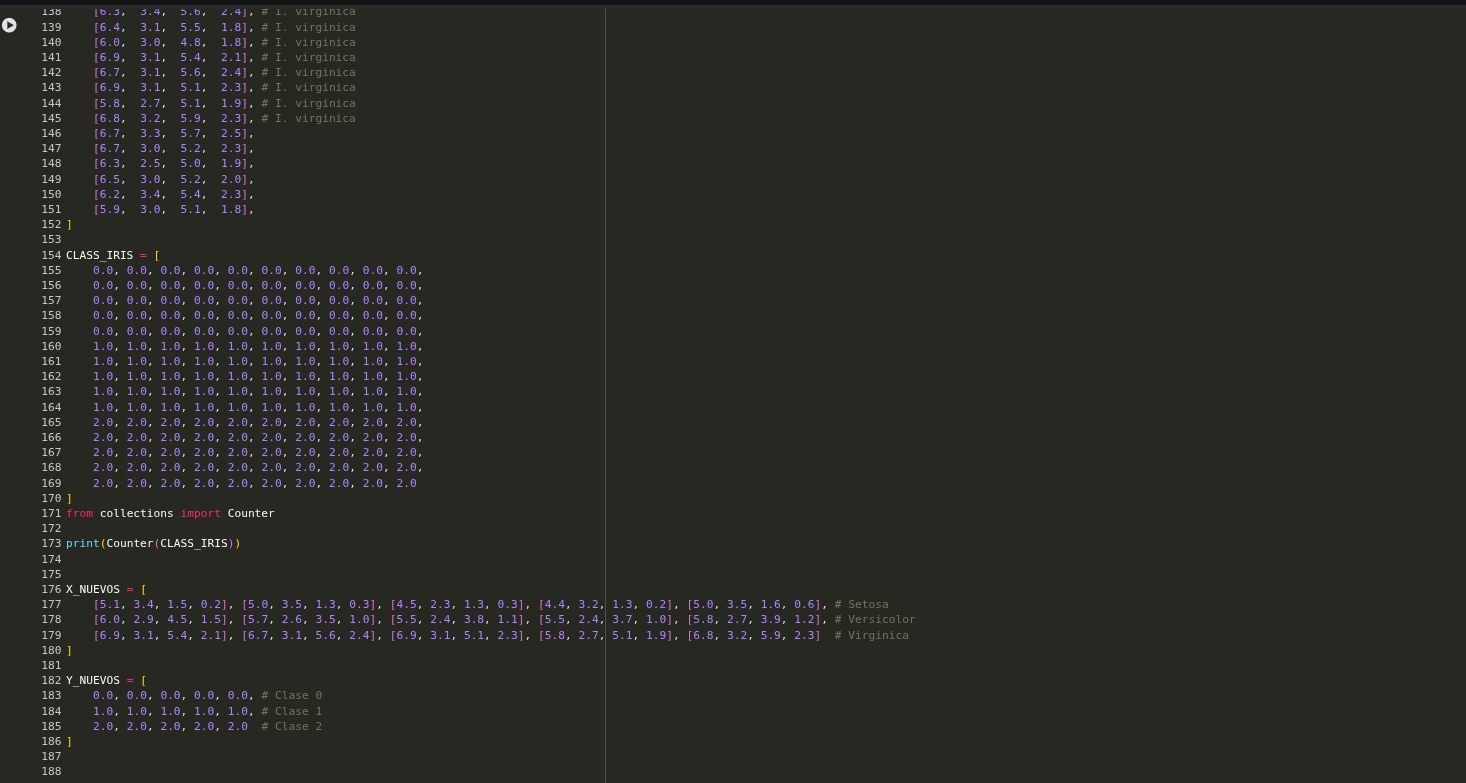
\includegraphics[width=0.7\textwidth]{img4.png} 
		\caption{Distribución y formato tabular del conjunto de datos Iris.}
		\label{fig:esquema_4}
	\end{figure}
	
	\subsection{Implementación en TensorFlow}
	La primera etapa experimental se desarrolló en \textbf{TensorFlow} empleando programación orientada a objetos. Esta estructura encapsula la lógica del modelo, facilitando la experimentación sistemática mediante la modificación de hiperparámetros.
	
	\begin{itemize}
		\item \textbf{Definición de la clase:} Se construye una clase orientada a objetos que hereda de las estructuras base del framework, configurando una capa densa de salida con activación \textit{Softmax}, idónea para resolver problemas de clasificación multiclase (mapeando las salidas a probabilidades para las 3 clases).		
		
		\begin{figure}[H]
			\centering
			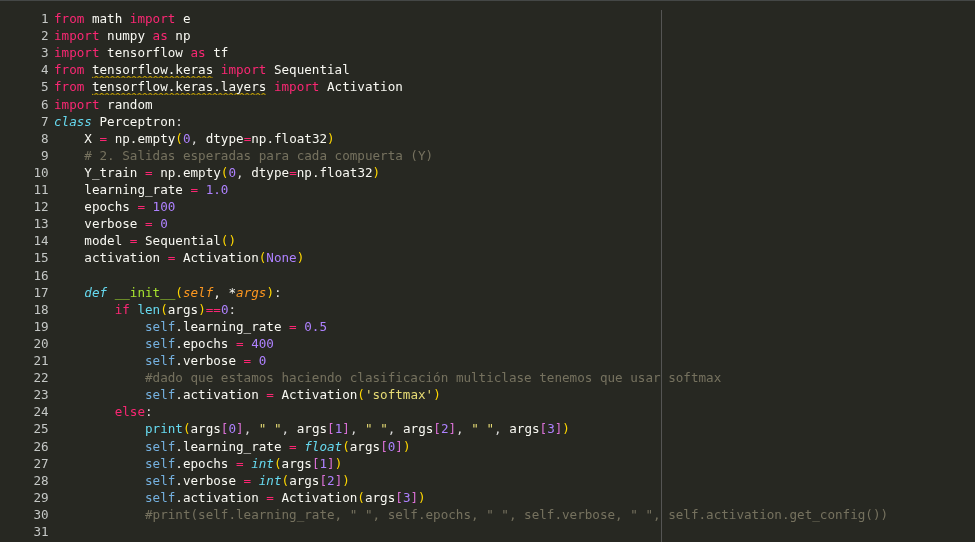
\includegraphics[width=0.7\textwidth]{img5.png} 
			\caption{Estructura orientada a objetos de la clase perceptrón en TensorFlow.}
			\label{fig:clase_perceptron}
		\end{figure}
		
		\item \textbf{Métodos principales:} La clase implementa funciones modulares para la carga de datos, definición de épocas, entrenamiento iterativo mediante optimizadores de descenso de gradiente y predicción final.
		
		\begin{figure}[H]
			\centering
			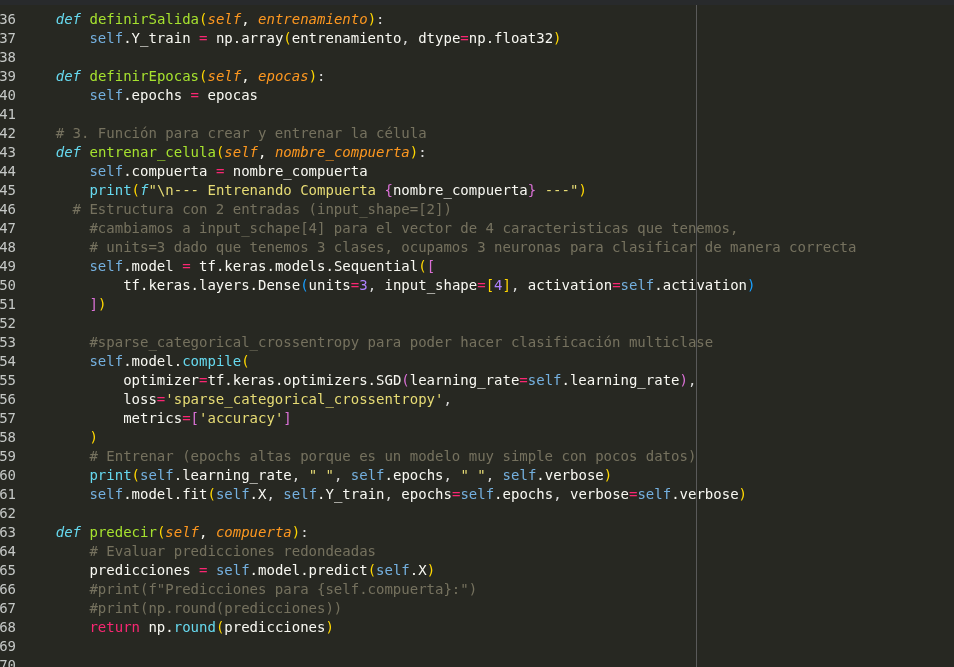
\includegraphics[width=0.7\textwidth]{img6.png} 
			\caption{Métodos de inicialización y control de entrenamiento en TensorFlow.}
			\label{fig:métodos_perceptron}
		\end{figure}
		
		\item \textbf{Prueba 1: Tasa de aprendizaje de 0.5 y 500 épocas.} Bajo esta configuración equilibrada, el modelo logra minimizar la función de pérdida de manera eficiente.
		
		\begin{figure}[H]
			\centering
			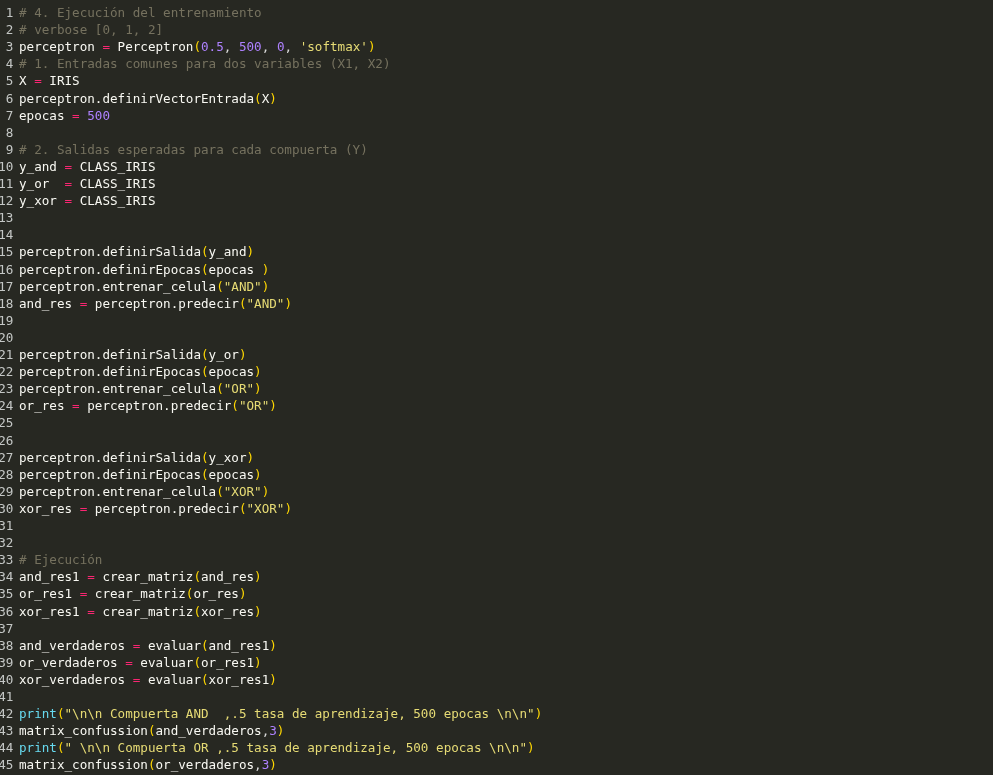
\includegraphics[width=0.7\textwidth]{img7.png} 
			\caption{Ejecución del entrenamiento con $\eta = 0.5$ y 500 épocas en TensorFlow.}
			\label{fig:entrenamiento_0.5_500}
		\end{figure}
		
		Las métricas obtenidas reflejan un rendimiento sobresaliente, clasificando correctamente el 100\% de las muestras de validación externas.
		
		\begin{figure}[H]
			\centering
			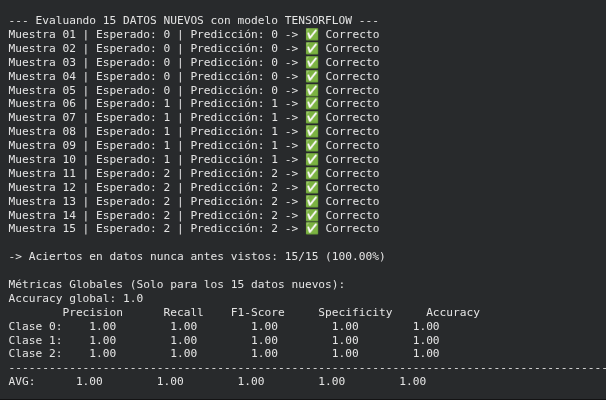
\includegraphics[width=0.7\textwidth]{img8.png} 
			\caption{Métricas de desempeño (Precision, Recall, F1-Score y Accuracy) para la Prueba 1.}
			\label{fig:resultados_prueba_1}
		\end{figure}
		
		\textbf{Análisis de resultados:} El éxito de esta prueba radica en la sinergia entre un número suficiente de épocas y una tasa de aprendizaje moderada, permitiendo que el optimizador encuentre los mínimos globales sin sobrepasar la región de convergencia.
		
		\item \textbf{Prueba 2: Tasa de aprendizaje de 0.5 y 50 épocas.} Reduciendo el número de iteraciones a una décima parte.
		
		\begin{figure}[H]
			\centering
			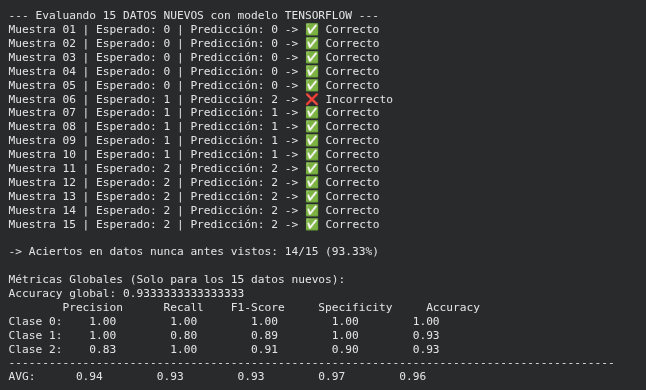
\includegraphics[width=0.7\textwidth]{img9.png} 
			\caption{Resultados con $\eta = 0.5$ y 50 épocas.}
			\label{fig:resultados_prueba_3}
		\end{figure}
		
		\textbf{Análisis:} Se observa una degradación notable en las métricas. La falta de épocas impide que los pesos sinápticos converjan a los valores óptimos, evidenciando un problema de subajuste (\textit{underfitting}).
		
		\item \textbf{Prueba 3: Tasa de aprendizaje de 0.7 y 5 épocas.} Configuración altamente restrictiva en tiempo y agresiva en actualización.
		
		\begin{figure}[H]
			\centering
			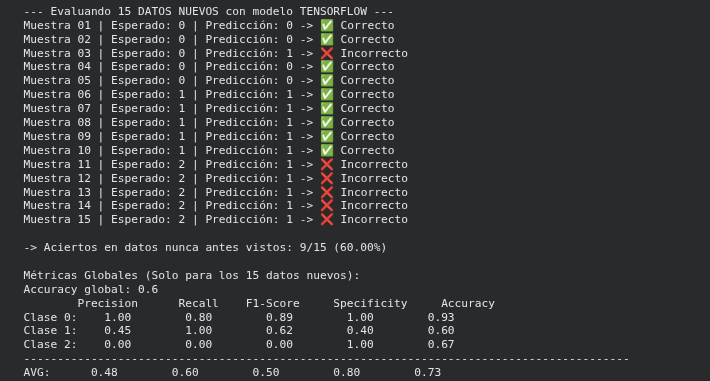
\includegraphics[width=0.7\textwidth]{img10.png} 
			\caption{Resultados con $\eta = 0.7$ y 5 épocas.}
			\label{fig:resultados_prueba_4}
		\end{figure}	
		
		\textbf{Análisis:} El rendimiento colapsa. Combinar un número ínfimo de épocas con una tasa de aprendizaje grande genera oscilaciones violentas en el espacio de pesos, impidiendo cualquier forma de aprendizaje útil.
	\end{itemize}
	
	\subsection{Implementación en PyTorch}
	La segunda fase implementa la misma arquitectura bajo \textbf{PyTorch}, utilizando módulos basados en `nn.Module` y optimizadores estocásticos con tensores explícitos.
	
	\begin{itemize}
		\item \textbf{Definición de la clase RedNeuronal:}
		
		\begin{figure}[H]
			\centering
			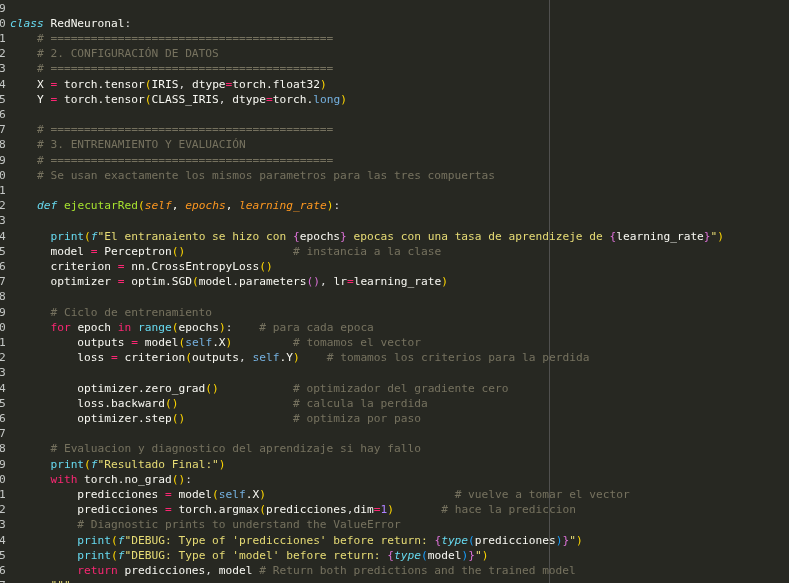
\includegraphics[width=0.7\textwidth]{img11.png} 
			\caption{Arquitectura y ciclo de entrenamiento orientado a objetos en PyTorch.}
			\label{fig:clase_pytorch}
		\end{figure}		
		
		\item \textbf{Prueba con 3000 épocas y tasa de 0.1:} Al extender las épocas y refinar el paso de aprendizaje, PyTorch logra una precisión global del $98\%$ en entrenamiento y un $100\%$ impecable en los 15 datos nuevos de validación.
		
		\begin{figure}[H]
			\centering
			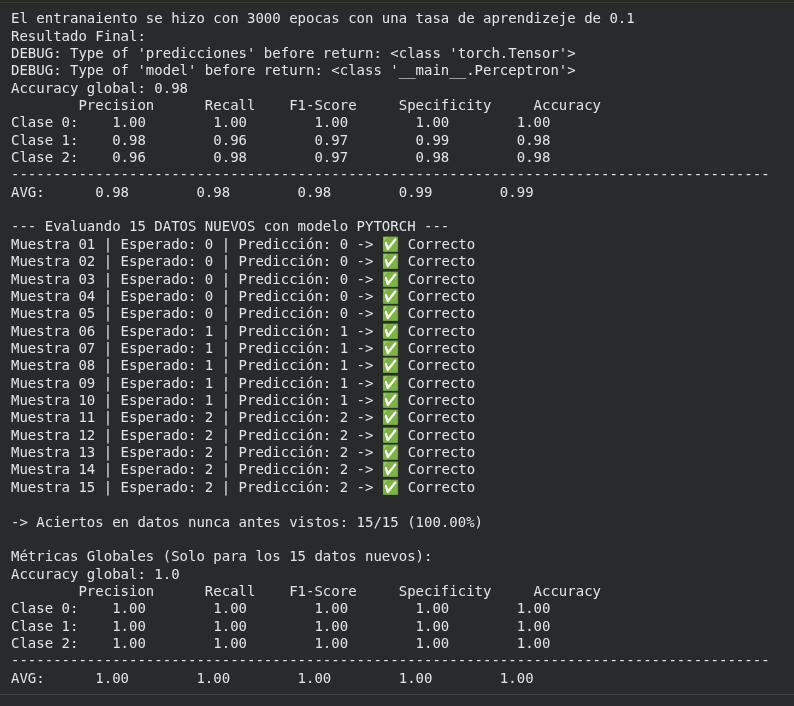
\includegraphics[width=0.7\textwidth]{img12.png} 
			\caption{Resultados de ejecución en PyTorch (3000 épocas, $\eta = 0.1$).}
			\label{fig:resultados_prueba5}
		\end{figure}		
		
		\item \textbf{Prueba con 500 épocas y tasa de 0.5:}
		
		\begin{figure}[H]
			\centering
			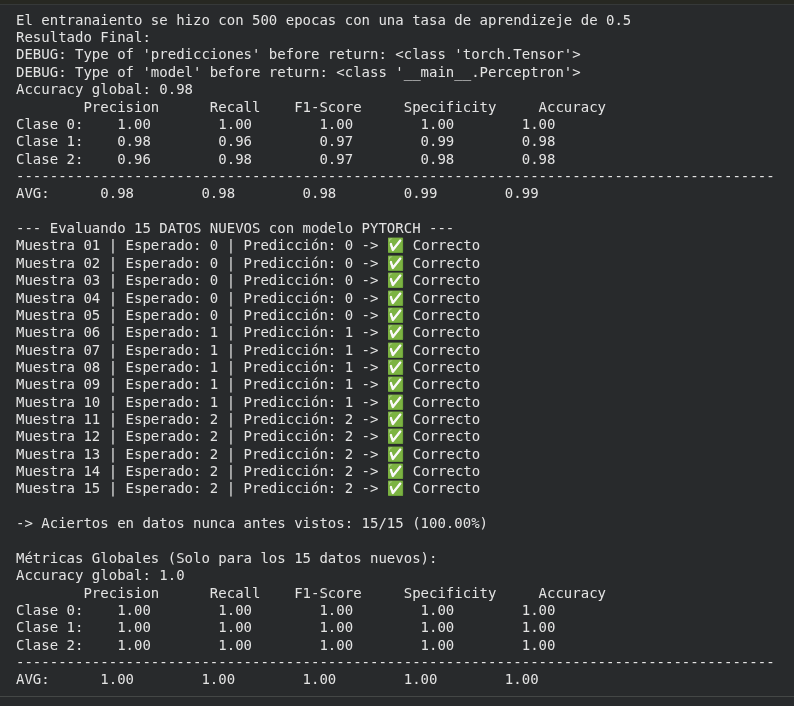
\includegraphics[width=0.7\textwidth]{img13.png} 
			\caption{Resultados de ejecución en PyTorch (500 épocas, $\eta = 0.5$).}
			\label{fig:resultados_prueba6}
		\end{figure}		
		
		\item \textbf{Prueba con 50 épocas y tasa de 0.7:}
		
		\begin{figure}[H]
			\centering
			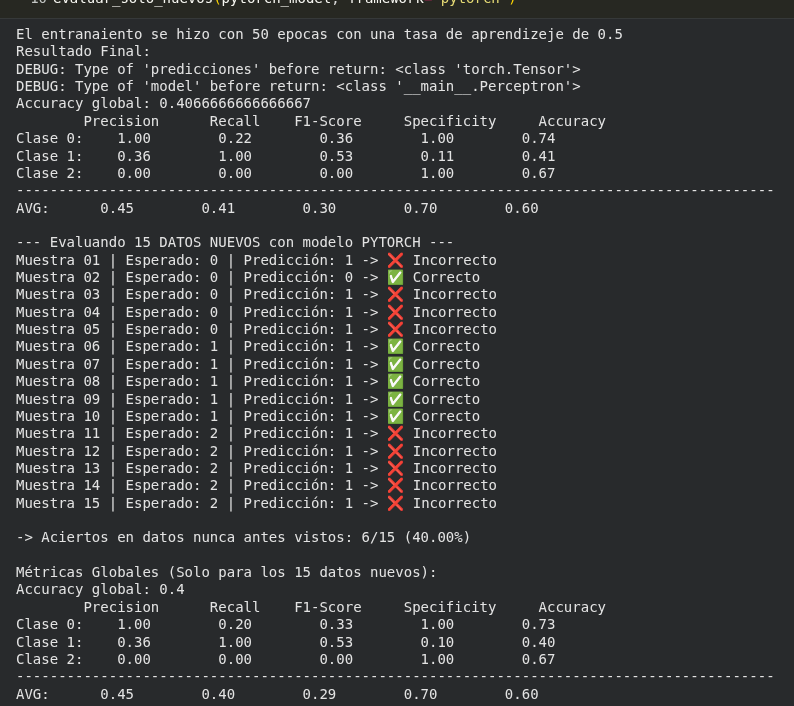
\includegraphics[width=0.7\textwidth]{img14.png} 
			\caption{Resultados de ejecución en PyTorch (50 épocas, $\eta = 0.7$).}
			\label{fig:resultados_prueba7}
		\end{figure}		
		
	\end{itemize}
	
	\subsection{Análisis Crítico de la Variación de Parámetros}
	El comportamiento observado en ambos frameworks demuestra que el rendimiento de un modelo neuronal no es estático, sino altamente sensible a dos hiperparámetros críticos:
	
	\begin{enumerate}
		\item \textbf{Tasa de Aprendizaje ($\eta$):} Regula la magnitud de las correcciones aplicadas a los pesos sinápticos en cada iteración del gradiente. 
		\begin{itemize}
			\item Si es \textit{demasiado baja}, el entrenamiento requiere un número impráctico de iteraciones y puede estancarse en mínimos locales secundarios.
			\item Si es \textit{demasiado alta} (como $0.7$ en pocas épocas), el optimizador sobrepasa constantemente el punto óptimo de convergencia, provocando divergencia numérica y oscilaciones erráticas en la función de pérdida.
		\end{itemize}
		\item \textbf{Número de Épocas:} Define el horizonte temporal de aprendizaje del modelo sobre el conjunto de datos completo. Un déficit de épocas trunca el proceso de minimización del error, mientras que un balance adecuado permite estabilizar los pesos sin incurrir necesariamente en sobreajuste debido a la simplicidad del dataset analizado.
	\end{enumerate}
	
	\newpage
	\section{Conclusiones}	
	A lo largo del desarrollo de esta práctica se cumplieron satisfactoriamente los objetivos planteados, logrando comprender y contrastar el comportamiento operativo de los perceptrones simples y multicapa aplicados a problemas de clasificación multiclase. Mediante el uso de TensorFlow y PyTorch, se evidenció que la implementación bajo un paradigma orientado a objetos otorga una alta modularidad, escalabilidad y claridad en la gestión de flujos de datos.
	
	Asimismo, los experimentos demostraron que el éxito en el rendimiento predictivo (reflejado en métricas de precisión, \textit{recall} y \textit{F1-score}) depende de forma directa de la sintonización adecuada de los hiperparámetros de entrenamiento. Se comprobó empíricamente que configuraciones desbalanceadas —como tasas de aprendizaje agresivas combinadas con un número insuficiente de épocas— destruyen la capacidad de convergencia del modelo, arrojando resultados deficientes, en contraste con configuraciones estables que alcanzan una generalización óptima del 100\% en datos no vistos.
	
	\newpage
	\section{Referencias}
	
	\begin{itemize}
		\item ``Iris Species'', Kaggle Dataset Repository. Accedido el 7 de septiembre de 2026. [En línea]. Disponible: https://www.kaggle.com/datasets/uciml/iris
		\item A. Paszke et al., ``PyTorch: An Imperative Style, High-Performance Deep Learning Library'', en \textit{Advances in Neural Information Processing Systems 32}, Curran Associates, Inc., 2019, pp. 8026-8037.
		\item M. Abadi et al., ``TensorFlow: A system for large-scale machine learning'', en \textit{12th USENIX Symposium on Operating Systems Design and Implementation (OSDI 16)}, 2016, pp. 265-283.
		\item F. Chollet, \textit{Deep Learning with Python}, 2.a ed. Manning Publications, 2021.
		\item S. Haykin, \textit{Neural Networks and Learning Machines}, 3.a ed. Pearson, 2008.
		\item F. Rosenblatt, ``The perceptron: A probabilistic model for information storage and organization in the brain'', \textit{Psychological Review}, vol. 65, no. 6, pp. 386-408, 1958.
	\end{itemize}
	
\end{document}
